\documentclass{article}
\usepackage[utf8]{inputenc}
\usepackage{amsmath}
\usepackage{amssymb}
\usepackage{graphicx}
\usepackage{tikz}
\usepackage{geometry}
 \geometry{
 a4paper,
 total={210mm,297mm},
 left=10mm,
 top=30mm,
 right=10mm
 }

\graphicspath{{./}}
\newcommand*\circled[1]{\tikz[baseline=(char.base)]{
    \node[shape=circle,draw,inner sep=0.5pt] (char) {#1};}}

\title{ 
\normalfont \large 
\textsc{Indian Institute of Technology, Ropar} \\    [40pt] 
\horrule{} \\[0.4cm] 
\Huge CS204 Course Project - Phase II\\ 
\horrule{} \\[0.5cm]
\protect\vspace{2.0cm}
\large
\textup{Team Members:}\\\vspace{1cm}
\begin{centering}
\begin{enumerate}
    \item Aditya Agarwal - 2019CSB1064
    \item Aneeket Mangal - 2019CSB1071
    \item Fadia Het Rakeshkumar - 2019CSB1084
    \item Shikhar Soni - 2019CSB1119
    \item Tanmay Aeron - 2019CSB1124
\end{enumerate}
\end{centering}
\date{}
\centering
\protect\vspace{4.0cm}

\includegraphics[width=1.0\textwidth]{riscv-logo-1.png}
}


\begin{document}
\maketitle
\newpage
\begin{centering}
\begin{Huge}
\textsf{Project Description}\\
\end{Huge}
\end{centering}
\protect\vspace{2.0cm}
\Large
The aim of this project is to simulate the machine level execution of RISC V 32-bit instructions using a high level language.\\

The Project also aims to give updates to the user regarding each step of the execution of the program. It also returns the final status of the memory and registers as output for the user to analyse the working of their programs thoroughly.\\

The Project currently allows the user to use 29 different instructions and can be extended to allow the use of any number of instructions by editing the .csv files as long as the instructions are supported by 32-bit RISC V ISA. \\

The program supports the use of `knobs' which will enable the user to select whether or not they want pipelining, data forwarding, and other details to be printed at the end of running the program.\\\\\\
The program executes each instruction using five stages as described in the RISC V architecture.\\

There are 5 separate knobs, all with a different purpose.\\
\begin{enumerate}
  \item {\bf Knob1:} Used to enable/disable pipelining during runtime. 
  \item {\bf Knob2:} Used to enable/disable data forwarding
  \item {\bf Knob3:} Used to enable/disable printing values in the register file at the end of each cycle.
  \item {\bf Knob4:} Used to enable/disable printing information in the pipeline registers at the end of each cycle, along with the cycle number.
  \item {\bf Knob5:} This is like enabling knob4 for a specific instruction. We will be able to see pipeline register for that particular instruction only.
\end{enumerate}\\
\newpage
\begin{centering}
\begin{Huge}
\begin{bf}
\vspace{2.0cm}
\textsf{Technologies employed}\\
\end{bf}
\end{Huge}
\end{centering}
\protect\vspace{2.0cm}
\textbf{}
\huge
Back-end - Python3
\begin{enumerate}
  \item {\bf pandas} for reading {\bf .csv} files.
  \item {\bf os} for getting and adding path to certain file locations.
  \item {\bf collections.defaultdict} to make a hash map for memory.
  \item {\bf sys} for reading and editing files with ease.
  \item {\bf termcolor.colored} for printing colored text in the terminal
\end{enumerate}\\
\textbf{}

Front-end - Python3
\begin{enumerate}
  \item {\bf PyQt5} for the Graphic User Interface.
  \item {\bf qdarkstyle} for dark theme in the GUI.
  \item {\bf json} for making dictionaries with ease in GUI
\end{enumerate}

\newpage
\begin{centering}
\begin{Huge}
\textsf{Implementation Details}\\
\end{Huge}
\end{centering}
\protect\vspace{1.0cm}
We have implemented the project using the following method:\\

First it takes the input from a \textsl{\textbf{.mc}} file that contains the input in the required format, the content of this file can be modified using the GUI editor or by changing the main.mc file.\\
Then, it stores the \textsl{\textbf{.data}} part into the data memory and the \textsl{\textbf{.text}} part in the text part of the memory.
Once that is completed, we run the program using the following method:
\begin{enumerate}
\item Instruction Fetch: PC is incremented by 4, and the instruction is loaded from the memory and stored in the Instruction Register.
\item Instruction Decode: We are identifying the instruction using the .csv file and {\bf pandas} library and returning all the required fields. The registers RA and RB are also set during this stage.
\item Execute: The ALU executes the instruction by computing the desired output using values stored in registers in RA, RB, imm, etc. The required type of ALU instruction is determined by another .csv file. We are updating the output in the RZ register.
\item Memory Access: Memory is read and written in this stage. This stage is used only for load and store instructions. For the remaining instructions, this stage is redundant. The value of the RY register is also consequently updated.
\item Register Write-back: Here we are storing the value of the temporary register RY in the destination register, resulting in the register files being updated. The register update is extremely fast compared to memory read and update.
\end{enumerate}
\newpage
We have implemented data forwarding by passing the required values from the source buffer to the destination buffer without the need of stalling in most cases. This helps to reduce the number of stalls required. The types of data forwarding are:
\begin{enumerate}
    \item Execute to Execute
    \item Memory to Execute
    \item Execute to Execute
\end{enumerate}
\\
\vspace{1cm}

\vspace{1cm}\\
The program detects hazards present which can cause an incorrect value to be register due to one instruction's stage being executed before another. This is fixed by either transferring data values directly with the help of data forwarding, or with the help of stalling which delays the next instruction so that the previous one is updated in time.\\\\
While data forwarding is enabled, there is no use of stalling\\ except for one particular case where we use it along with \\Memory-to-Execute data forwarding.

\newpage
\begin{centering}
\begin{Huge}
\textsf{Input/Output format details}\\
\end{Huge}
\vspace{0.6cm}
\end{centering}
\noindent
\Large
{\bf Input Format:}\\\\
0x0 0x00500513\\
0x4 0x008000EF\\
0x8 0x0440006F\\
\$\\
0x10000000 0x64\\\\
The input is given through GUI if the GUI is run else it is taken from the input file.\\\\
The section given before the `\$' sign is the text segment of the code and all the lines after it signify the data segment of the code.\\\\
Output is generated in the `generated' folder. It contains the following things  \\
\begin{enumerate}
    \item `registers.txt' contains the register values
    \item `memory.txt' contains the data part of the memory
    \item 'stats.txt' contains the statistical details of the program
    \item `outputLog.txt' contains the buffer data of each cycle
\end{enumerate}


\newpage
\textbf{In \textsl{stats.txt} we have printed the following:}

\begin{enumerate}
\begin{LARGE}
\item \textsf{Total number of cycles}
\item \textsf{Total number of instructions executed}
\item \textsf{CPI}
\item \textsf{Data Transfer instructions executed}
\item \textsf{ALU instructions executed}
\item \textsf{Control instructions executed}
\item \textsf{Total Stall Count}
\item \textsf{Number of Data Hazards}
\item \textsf{Total Control Hazards}
\item \textsf{Total Branch misprediction}
\item \textsf{Number of stalls due to data hazards}
\item \textsf{Number of stalls due to control hazards}
\end{LARGE}
\end{enumerate}

\par\noindent\rule{\textwidth}{0.4pt}



\noindent
\textbf{An example output for \textsl{stats.txt} is :}\\
\\
\begin{LARGE}
\textsf{Total number of Cycles in the program :14}\\
\textsf{Total number of Instructions executed :4}\\
\textsf{CPI is :3.5}\\
\textsf{Data Transfer Instructions Executed :0}\\
\textsf{ALU instructions are :4}\\
\textsf{Contol instructions :0}\\
\textsf{Total Stall Count are :6}\\
\textsf{Number of Data Hazards are :3}\\
\textsf{Total Control Hazards are :0}\\
\textsf{Total Branch mispredictions are :0}\\
\textsf{Number of stalls due to data hazards are :6}\\
\textsf{Number of stalls due to control hazards are :0}\\\\
\textsf{The instruction fed was:}\\
\textsf{0x0	0x00A50513}\\
\textsf{0x4	0x00A50513}\\
\textsf{0x8	0x00A50513}\\
\textsf{0xC	0x00A50513}\\
\end{LARGE}
\vspace{0.6cm}

\noindent
\newpage
\begin{centering}
\begin{Huge}
\textsf{Graphical User Interface}\\
\end{Huge}
\vspace{1cm}
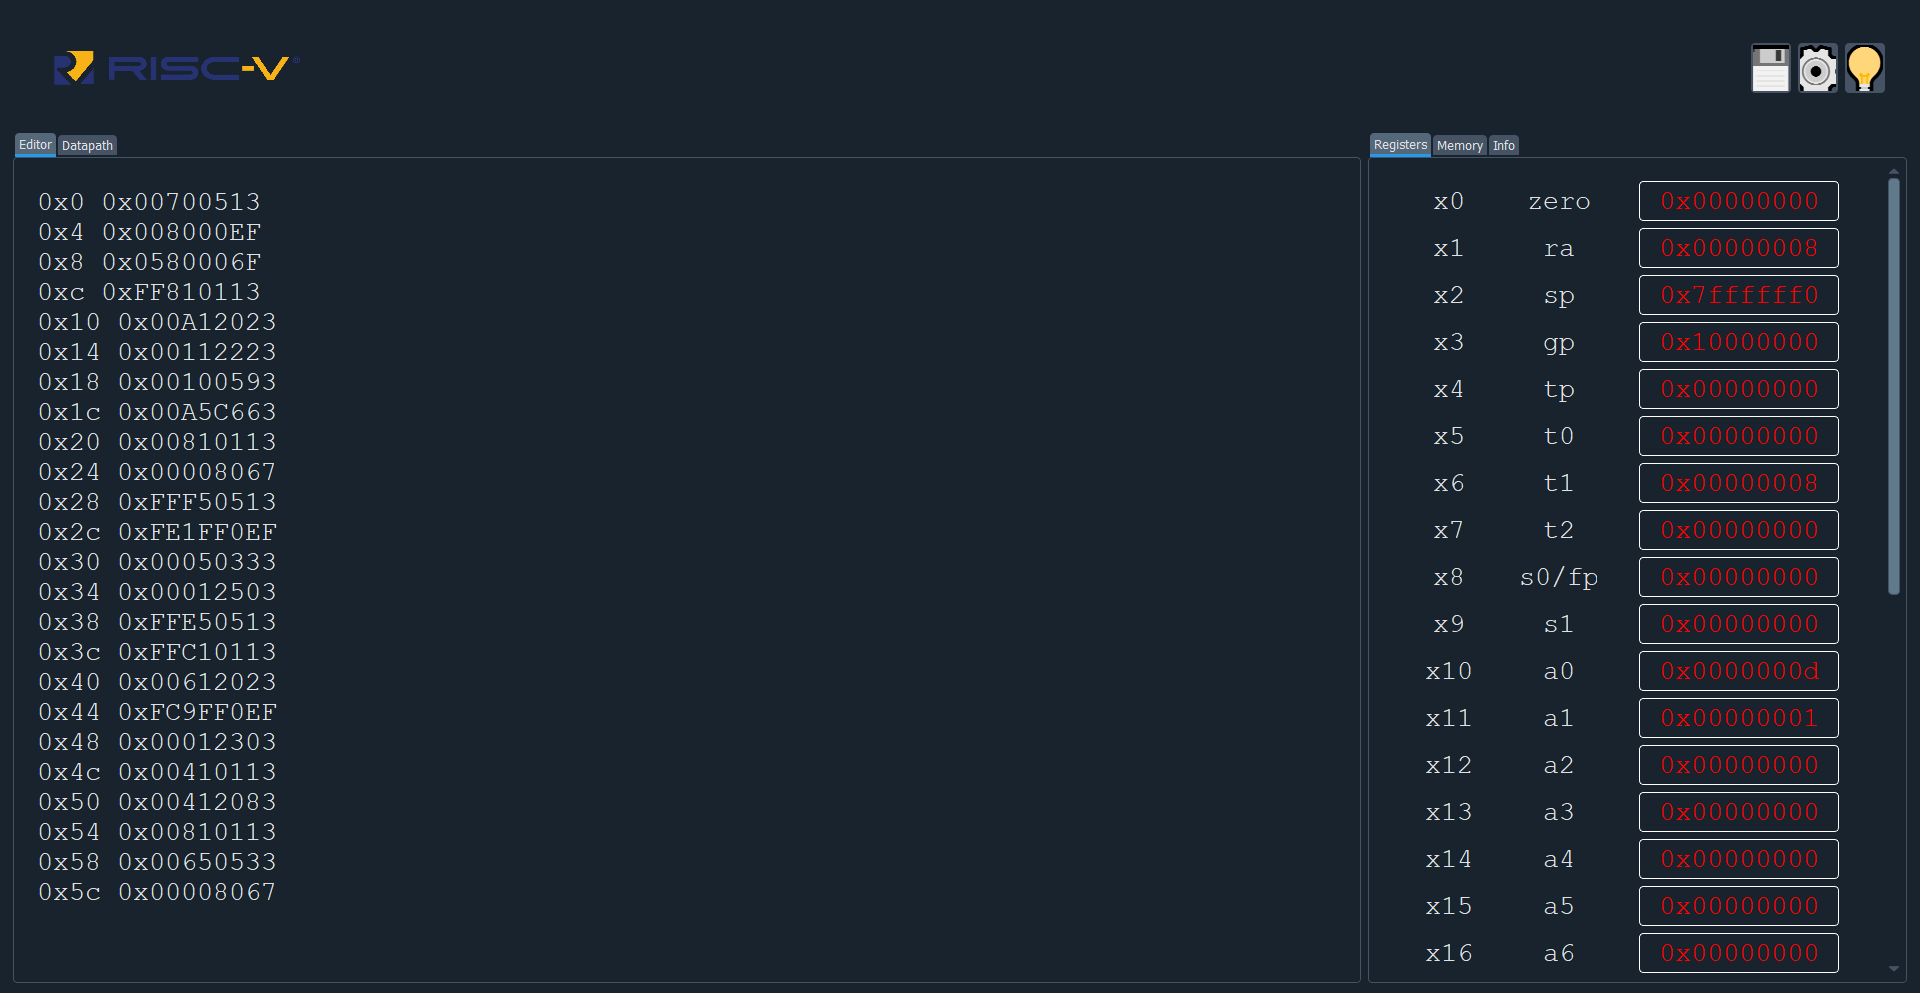
\includegraphics[width=1.0\textwidth]{pic4.png}\vspace{2cm}
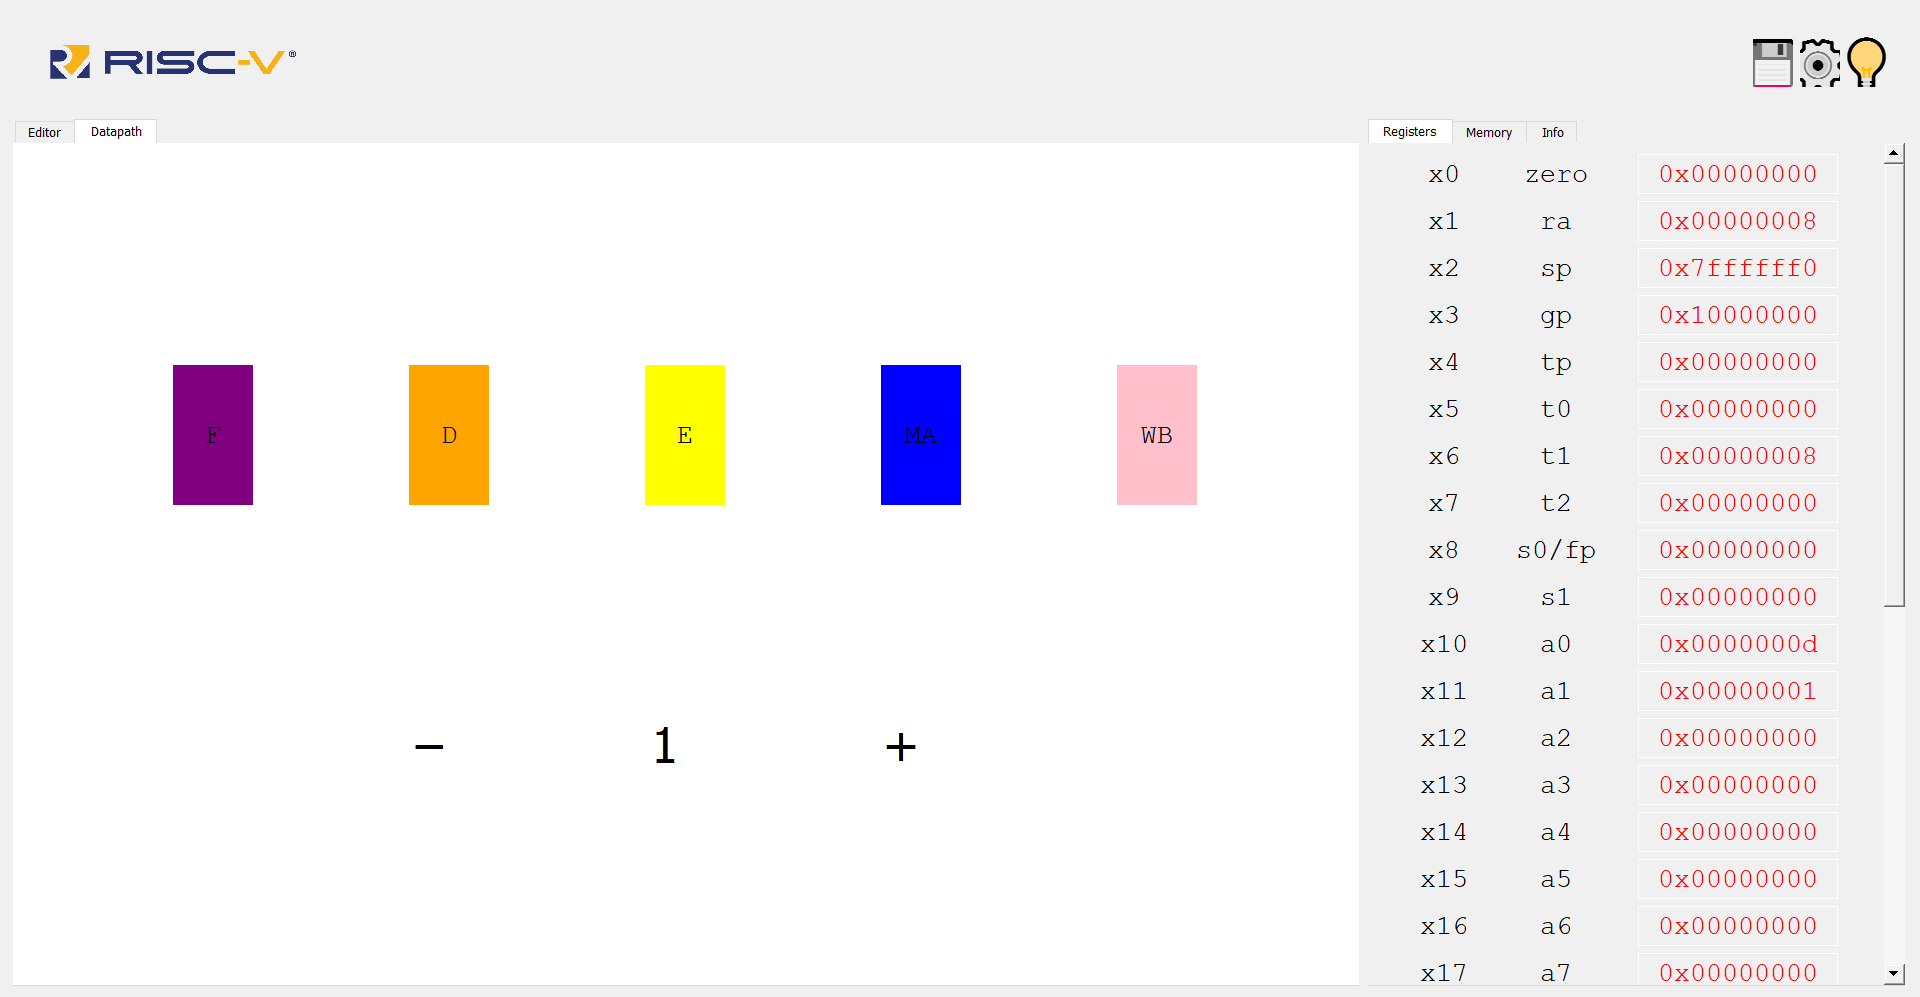
\includegraphics[width=1.0\textwidth]{pic6.png}
\newpage

\begin{centering}
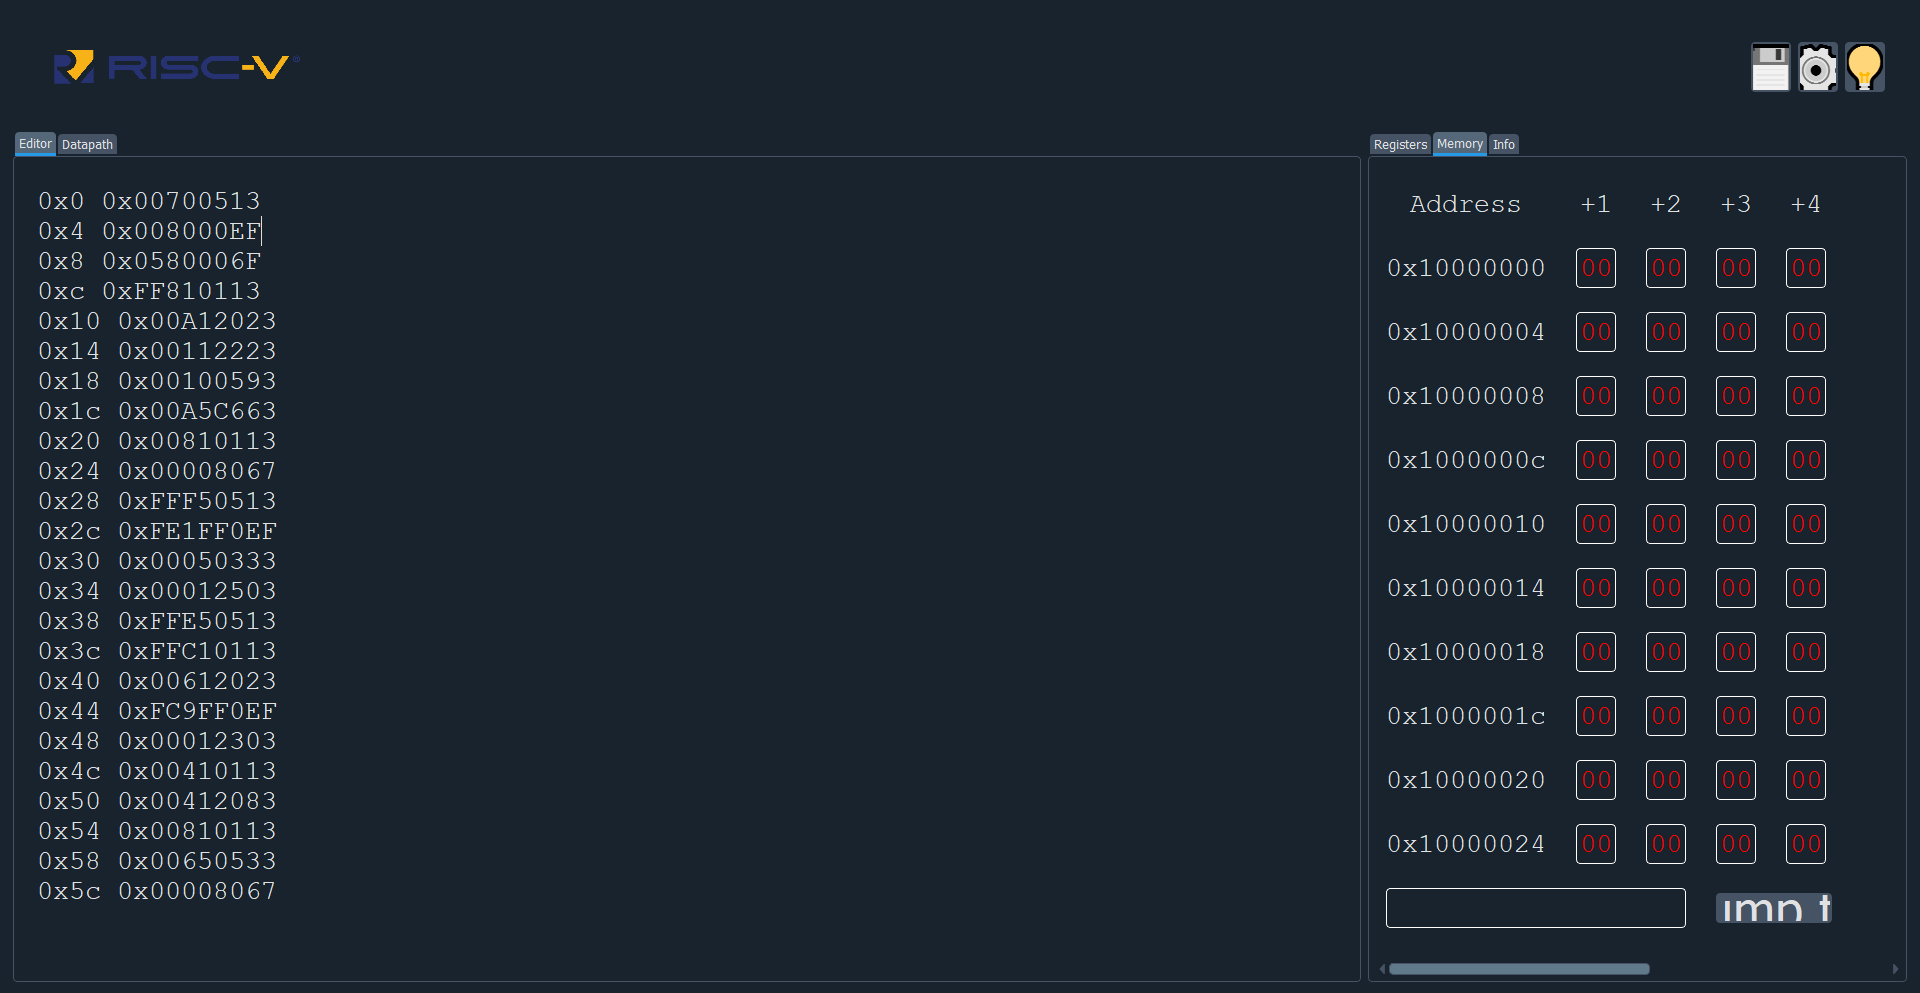
\includegraphics[width=1.0\textwidth]{pic5.png}
\end{centering}
\\\\
\end{centering}
\vspace{3cm}
\LARGE
Here we can see the jump to register functionality, where we have stored a value in the register 0x10000500, and are jumping to it and seeing the value.\\

For example to jump on the location 0x10000500 write 10000500 in the Jump to box which is in the bottom right in the memory tab.
\newpage
\def\checkmark{\tikz\fill[scale=0.4](0,.35) -- (.25,0) -- (1,.7) -- (.25,.15) -- cycle;}
\LARGE
\\\\
We have made the GUI in both light and dark theme. The theme can be changed by clicking on the "yellow bulb" which can be seen in the top right corner.

We have shown memory, registers and info on the right section of the GUI while on the left part there is Code Editor.
In the Code Editor you can edit your code or copy paste your code and also save it.
The info contains the details of the instruction being executed in each stage during a
cycle.
First of all we will paste the code in the Editor on the left side and then save and compile the code by clicking the respective `save' button which is the first button on the top right and `compile' button. The code will get updated in \textsl{\textbf{main.mc}} file and then the code will be executed and a \checkmark\hspace{0.7mm} will appear. The memory and registers will be updated simultaneously.\\

\begin{itemize}
    \item We can jump to the memory using the `Jump to' box on the bottom right corner in the memory section.
    \item All the registers can be seen in the register file by scrolling in the register file section.
    \item Executing \textsl{\textbf{main.py}} always generates a GUI window where you can code in the Editor.
    \item We can also execute non GUI code by writing\textrightarrow   python main.py
    \item The DataPath explains how the data is flowing through each stage.
    \item Here the 5 stages can be seen in the DataPath tab.
    \item The number below it is the cycle number for which the DataPath is shown.
    \item You can see the DataPath in the respective cycle by going to that cycle.
    \item Click on + to go to the next cycle and on - to go to the previous cycle.
\end{itemize}

\end{document}



